\documentclass[12pt,a4paper,oneside]{report}

% =========================================================
% LINGUA, CODIFICA, FONT
% =========================================================
\usepackage[utf8]{inputenc}
\usepackage[T1]{fontenc}
\usepackage[italian]{babel}

% Font stile Times/Times New Roman, compatibile con pdfLaTeX
\usepackage{newtxtext}
\usepackage{newtxmath}

% Migliora la resa tipografica e la giustificazione
\usepackage{microtype}

% =========================================================
% IMPAGINAZIONE
% =========================================================
\usepackage[
    a4paper,
    left=2.7cm,
    right=2.7cm,
    top=2.6cm,
    bottom=2.6cm,
    includeheadfoot
]{geometry}

% Interlinea: le linee guida indicano 1.15 o 1.5.
% Uso 1.15 per una versione PDF più compatta e uniforme.
\usepackage{setspace}
\setstretch{1.15}

% Rientro dei paragrafi
\setlength{\parindent}{1.25cm}
\setlength{\parskip}{0pt}
\usepackage{indentfirst}

% Pagine bianche senza intestazioni/numeri
\usepackage{emptypage}

% =========================================================
% NUMERAZIONE PAGINE
% =========================================================
\usepackage{fancyhdr}
\pagestyle{fancy}
\fancyhf{}

% Numero pagina centrato: stabile in lettura PDF/oneside.
\fancyfoot[C]{\thepage}

\renewcommand{\headrulewidth}{0pt}
\renewcommand{\footrulewidth}{0pt}

\fancypagestyle{plain}{
    \fancyhf{}
    \fancyfoot[C]{\thepage}
    \renewcommand{\headrulewidth}{0pt}
    \renewcommand{\footrulewidth}{0pt}
}

% =========================================================
% TITOLI DEI CAPITOLI E SEZIONI
% =========================================================
\usepackage{titlesec}

% Capitoli nello stile: "1 Introduzione", senza scritta "Capitolo"
\titleformat{\chapter}[hang]
    {\normalfont\huge\bfseries}
    {\thechapter}
    {1em}
    {}

\titlespacing*{\chapter}{0pt}{-5pt}{25pt}

% Profondità numerazione e indice
\setcounter{secnumdepth}{3}
\setcounter{tocdepth}{2}

% =========================================================
% FIGURE, TABELLE, DIDASCALIE
% =========================================================
\usepackage{graphicx}
\graphicspath{{figures/}{img/}}

\usepackage{float}
\usepackage{subcaption}

\usepackage{caption}
\DeclareCaptionLabelSeparator{dot}{. }

% Didascalie simili alla tesi di esempio: Figura 1. ...
\captionsetup{
    font=small,
    labelfont=it,
    textfont=it,
    labelsep=dot
}

% Tabelle
\usepackage{booktabs}
\usepackage{array}
\usepackage{longtable}
\usepackage{multirow}
\usepackage{tabularx}
\usepackage{tikz}
\usetikzlibrary{arrows.meta,positioning,shapes.geometric,fit,calc}
\usepackage{pgfplots}
\pgfplotsset{compat=1.18}

% =========================================================
% MATEMATICA E UNITÀ DI MISURA
% =========================================================
\usepackage{amsmath}
\let\Bbbk\relax
\usepackage{amssymb}

% Equazioni numerate per capitolo: (2.1), (2.2), ...
\numberwithin{equation}{chapter}

% siunitx non è sempre presente nella distribuzione TeX installata localmente.
% Se vuoi usarlo, installa texlive-science oppure riattiva questo blocco.
\IfFileExists{siunitx.sty}{
    \usepackage{siunitx}
    \sisetup{
        locale=DE,
        detect-all,
        per-mode=symbol
    }
}{}

% =========================================================
% ELENCHI
% =========================================================
\usepackage{enumitem}
\setlist{
    noitemsep,
    topsep=4pt
}

% =========================================================
% CODICE
% =========================================================
\usepackage{xcolor}
\usepackage{listings}

\lstdefinestyle{tesiCode}{
    basicstyle=\ttfamily\small,
    breaklines=true,
    frame=single,
    numbers=left,
    numberstyle=\tiny,
    captionpos=b,
    tabsize=4,
    showstringspaces=false
}

\lstset{style=tesiCode}

\renewcommand{\lstlistingname}{Listato}
\renewcommand{\lstlistlistingname}{Elenco dei listati}

% =========================================================
% BIBLIOGRAFIA
% =========================================================
% Crea un file bibliografia.bib nella stessa cartella del main.tex
\usepackage{csquotes}
\usepackage[
    backend=biber,
    style=alphabetic,
    sorting=nyt
]{biblatex}

\addbibresource{bibliografia.bib}

% Per usare riferimenti stile [CabLZ16], sostituire:
% style=numeric
% con:
% style=alphabetic

% =========================================================
% LINK E RIFERIMENTI INCROCIATI
% =========================================================
\usepackage{xurl}

\usepackage[
    hidelinks
]{hyperref}

\usepackage[italian,nameinlink,noabbrev]{cleveref}

\crefname{chapter}{capitolo}{capitoli}
\Crefname{chapter}{Capitolo}{Capitoli}
\crefname{section}{paragrafo}{paragrafi}
\Crefname{section}{Paragrafo}{Paragrafi}
\crefname{figure}{figura}{figure}
\Crefname{figure}{Figura}{Figure}
\crefname{table}{tabella}{tabelle}
\Crefname{table}{Tabella}{Tabelle}
\crefname{equation}{equazione}{equazioni}
\Crefname{equation}{Equazione}{Equazioni}
\crefname{lstlisting}{listato}{listati}
\Crefname{lstlisting}{Listato}{Listati}

% =========================================================
% DATI FRONTESPIZIO
% =========================================================
\usepackage{etoolbox}

\newcommand{\TesiTitolo}{Controllo semaforico adattivo mediante strategie Max-Pressure: progettazione e valutazione tramite simulazione}
\newcommand{\TesiCandidato}{Jakub Pawel Homoncik}
\newcommand{\TesiRelatore}{Prof. Giacomo Cabri}

% Lascia vuoto se non hai correlatori
\newcommand{\TesiCorrelatori}{}
% Esempio:
% \newcommand{\TesiCorrelatori}{Prof.ssa Manuela Montangero}

\newcommand{\TesiAnnoAccademico}{2025--2026}

\hypersetup{
    pdftitle={\TesiTitolo},
    pdfauthor={\TesiCandidato},
    pdfsubject={Controllo semaforico adattivo},
    pdfkeywords={Sistemi di trasporto intelligenti, Controllo semaforico adattivo, Simulazione, Max-Pressure, SUMO}
}

% Finche' le sezioni sono vuote, questo segnaposto crea un paragrafo
% invisibile e permette a LaTeX di interrompere correttamente la pagina.
% I richiami possono essere rimossi man mano che viene inserito il testo.
\newcommand{\tesischeletro}{\mbox{}\par}

% I capitoli successivi a Manhattan restano nel sorgente come traccia di
% lavoro, ma non vengono compilati finche' non sono stati redatti.
\newif\ifcapitolifuturi
\capitolifuturitrue

% =========================================================
% FRONTESPIZIO
% =========================================================
\newcommand{\frontespizio}{
    \begin{titlepage}
        \thispagestyle{empty}
        \centering

        
\includegraphics[width=0.72\textwidth]{Logo_A_Positivo_Colore}\par

        \vspace{0.7cm}

        {\large
        Dipartimento di Scienze Fisiche, Informatiche e Matematiche
        \par}

        \vspace{0.5cm}

        {\large
        Corso di Laurea in Informatica
        \par}

        \vfill

        {\LARGE\bfseries
        \TesiTitolo
        \par}

        \vfill

        \begin{minipage}[t]{0.45\textwidth}
            \raggedright
            \textbf{Relatore:}\par\vspace{0.2cm}
            \TesiRelatore

            \ifdefempty{\TesiCorrelatori}
            {}
            {
                \par\vspace{0.8cm}
                \textbf{Correlatori:}\par\vspace{0.2cm}
                \TesiCorrelatori
            }
        \end{minipage}
        \hfill
        \begin{minipage}[t]{0.45\textwidth}
            \raggedleft
            \textbf{Candidato:}\par\vspace{0.2cm}
            \TesiCandidato
        \end{minipage}

        \vfill

        {\large
        Anno Accademico \TesiAnnoAccademico
        \par}

    \end{titlepage}

    \cleardoublepage
}

% =========================================================
% ESEMPIO DI USO DOPO \begin{document}
% =========================================================
\begin{document}

\hypersetup{pageanchor=false}
\frontespizio
\hypersetup{pageanchor=true}
\pagenumbering{roman}

\chapter*{Sommario}
\addcontentsline{toc}{chapter}{Sommario}

Il controllo semaforico a tempi fissi non utilizza informazioni sul traffico
osservato e può quindi assegnare il verde a direzioni poco richieste mentre si
formano code su altri accessi. Questa tesi studia strategie di controllo
adattivo basate sul principio Max-Pressure, nel quale ogni incrocio seleziona
la fase da servire confrontando le code a monte e a valle dei movimenti
consentiti. Il lavoro comprende una piattaforma sperimentale riproducibile
basata su SUMO e TraCI, un controller Max-Pressure con sette estensioni
specialistiche e una pipeline per analisi di ablazione, esecuzioni parallele e
produzione automatica di metriche e report.

La prima valutazione completa riguarda una rete sintetica Manhattan \(8
\times 8\), tre livelli di domanda e cinque seed. I 135 casi sperimentali sono
terminati senza errori e con censura nulla. Rispetto al programma semaforico
statico nativo, il miglior controller riduce il tempo medio di attesa del
\(64{,}26\%\) nel traffico leggero, del \(60{,}09\%\) nel traffico medio e del
\(53{,}05\%\) nel traffico elevato. I risultati mostrano inoltre che
l'aggiunta di una regola specialistica non produce necessariamente un
beneficio: alcune estensioni migliorano soltanto in specifici regimi, altre
rimangono inattive oppure introducono un costo superiore al vantaggio
ottenuto.

La seconda valutazione riguarda la rete reale di Bologna, con tre
distribuzioni della domanda, tre livelli di traffico e tre seed. In questo
scenario il Max-Pressure puro risulta sempre peggiore del programma semaforico
nativo. Sono stati quindi sviluppati due controller ibridi che conservano il
piano esistente nei regimi appropriati e attivano Max-Pressure in base al
carico osservato. Nelle 270 simulazioni considerate, completate senza censura,
è sempre uno dei due ibridi a ottenere la minore attesa media:
\texttt{mp\_super} prevale in cinque gruppi e \texttt{mp\_program0} in
quattro. Il risultato mostra che, su una rete reale, l'adattività può essere
più efficace quando integra il piano nativo anziché sostituirlo
continuamente.

\chapter*{Parole chiave}
\addcontentsline{toc}{chapter}{Parole chiave}

\begin{itemize}
    \item Sistemi di trasporto intelligenti;
    \item Controllo semaforico adattivo;
    \item Simulazione;
    \item Max-Pressure;
    \item SUMO.
\end{itemize}

\cleardoublepage
\tableofcontents
\cleardoublepage

\pagenumbering{arabic}
\chapter{Introduzione}
\label{chap:introduzione}

La regolazione semaforica decide come distribuire tra flussi in conflitto una
risorsa limitata, il diritto di attraversare un incrocio. Una scelta
apparentemente locale può propagarsi lungo la rete:
un verde troppo breve lascia una coda residua, un verde inutile sottrae tempo
agli altri accessi e una coda che raggiunge l'incrocio precedente può impedire
movimenti altrimenti non conflittuali. Per questo motivo il controllo dei
semafori costituisce un problema centrale nei sistemi di trasporto
intelligenti.

Questo capitolo introduce il problema affrontato, gli obiettivi e i contributi
del lavoro. La trattazione rimane volutamente ad alto livello, le formulazioni
matematiche, le scelte implementative e il protocollo sperimentale vengono
sviluppati nei capitoli successivi.

\section{Contesto e motivazioni}

I piani semaforici a tempi fissi sono semplici, prevedibili e poco costosi da
gestire. Associano a ciascuna fase una durata definita in anticipo e
ripetono ciclicamente la stessa sequenza. La loro efficacia dipende tuttavia
dalla corrispondenza tra il profilo di domanda usato durante la progettazione e
il traffico effettivamente presente. Quando la domanda cambia nello spazio o
nel tempo, il piano può continuare a servire una direzione vuota mentre su un
altro accesso si accumulano veicoli.

Il controllo adattivo cerca invece di usare osservazioni correnti della rete
per modificare il servizio offerto. Tra le strategie decentralizzate, il
Max-Pressure è particolarmente interessante perché non richiede una previsione
completa della domanda né un unico ottimizzatore centrale. Ogni intersezione
confronta le code a monte e a valle dei movimenti consentiti e assegna il verde
alla fase con pressione maggiore. Questa famiglia deriva dalle politiche di
backpressure per reti di code \cite{tassiulas1992stability}, nel traffico
urbano, la letteratura ha mostrato importanti proprietà di stabilità e
throughput in opportune ipotesi modellistiche
\cite{varaiya2013maxpressure,wongpiromsarn2012distributed,levin2023review}.

Il passaggio dalla teoria a una simulazione microscopica realistica introduce
però costi e vincoli che il modello ideale tende a semplificare: giallo e
tempo di sgombero, minimo e massimo verde, capacità finita delle corsie,
spillback, arrivi a plotoni e necessità di non trascurare movimenti deboli. Ne
segue che ``scegliere sempre la pressione massima'' non è, da solo, una
specifica sufficiente per un controller utilizzabile.

\section{Problema affrontato}

Il lavoro affronta due problemi collegati. Il primo è ingegneristico: costruire
una piattaforma con cui implementare, eseguire e confrontare in modo
riproducibile controller semaforici diversi su reti SUMO sintetiche e reali. Il
secondo è sperimentale: stabilire in quali condizioni il Max-Pressure di base
o le sue estensioni migliorino effettivamente il flusso rispetto a un programma
statico.

L'indicatore principale è il tempo di attesa, affiancato da tempo di viaggio,
perdita di tempo, velocità, numero di viaggi completati e censura. Il lavoro
non persegue obiettivi ambientali: consumi di carburante ed emissioni non sono
utilizzati per selezionare o valutare i controller. In questo modo l'analisi
rimane allineata alla domanda di ricerca, concentrata sull'efficienza degli
incroci e del flusso veicolare.

Una difficoltà metodologica importante è evitare conclusioni ottenute da un
solo seed o da una simulazione interrotta prima che tutti i veicoli completino
il viaggio. Un controller può mostrare una bassa attesa media semplicemente
perché i veicoli più problematici sono ancora nella rete. Per questo la
piattaforma registra esplicitamente la quota di viaggi non conclusi e considera
la censura una condizione necessaria per interpretare correttamente le altre
metriche.

\section{Obiettivi del lavoro di tesi}

Gli obiettivi sono i seguenti:

\begin{enumerate}
    \item implementare un controller Max-Pressure decentralizzato compatibile
    con le logiche semaforiche presenti nelle mappe SUMO;
    \item introdurre estensioni mirate a switching loss, minimo verde dinamico,
    fairness, capacità downstream, spillback e arrivi a plotoni;
    \item realizzare una pipeline di ablation che generi popolazioni
    riproducibili, esegua casi in parallelo e produca report confrontabili;
    \item definire metriche capaci di distinguere un reale miglioramento da un
    risultato condizionato da viaggi incompleti;
    \item valutare separatamente le varianti su una rete Manhattan regolare,
    prima di affrontare la maggiore eterogeneità della rete di Bologna;
    \item ricavare dai risultati indicazioni progettuali per controller capaci
    di adattarsi a regimi di traffico differenti.
\end{enumerate}

\section{Contributi del lavoro}

Il lavoro è partito da una base software composta dal collegamento con SUMO, da
un runner, da un generatore di popolazioni e da un controller fisso, che sono
stati poi integrati ed estesi con:

Nel seguito, con \emph{campagna sperimentale} si intende un insieme organizzato
di simulazioni eseguite con una stessa configurazione generale, variando in modo
controllato mappa, livello di domanda, seed e scenario di controllo.

\begin{itemize}
    \item un'implementazione completa del Max-Pressure, comprensiva di macchina
    a stati per preservare giallo e all-red;
    \item sette famiglie di estensioni parametriche e relativi contatori di
    attivazione;
    \item una rappresentazione uniforme degli scenari sperimentali e dei
    profili di guida;
    \item una pipeline batch con preflight, cache delle popolazioni,
    parallelismo, tracciamento del progresso e report automatici;
    \item il calcolo esplicito di viaggi completati e censura a partire dai file
    \texttt{tripinfo};
    \item una campagna finale su Manhattan $8\times8$ composta da 135
    simulazioni valide, tre livelli di domanda e cinque seed;
    \item l'estensione successiva della metodologia a distribuzioni spaziali
    non uniformi e a controller ibridi per la rete reale di Bologna.
\end{itemize}

Il contributo non consiste quindi soltanto in un algoritmo, ma in un processo
sperimentale osservabile. I contatori interni consentono di verificare se una
variante ha prodotto un risultato perché il suo meccanismo si è attivato o se,
al contrario, è rimasta operativamente identica al Max-Pressure di base.

\section{Organizzazione della tesi}

Il \cref{chap:stato-arte} presenta il controllo semaforico adattivo, il
Max-Pressure e gli strumenti di simulazione. Il \cref{chap:progettazione}
definisce requisiti e architettura della piattaforma. Il
\cref{chap:implementazione} descrive l'implementazione del controller e delle
estensioni. Il \cref{chap:metodologia} formalizza il protocollo sperimentale,
le popolazioni e le metriche. Il \cref{chap:manhattan} analizza la campagna
Manhattan $8\times8$. La parte successiva della tesi applica le indicazioni
ricavate alla rete di Bologna, introduce i controller ibridi sviluppati per la
mappa reale e discute i risultati conclusivi.


\chapter{Contesto e stato dell'arte}
\label{chap:stato-arte}

Per collocare il contributo è utile distinguere tre livelli:
le strategie di controllo già note in letteratura, gli strumenti software
utilizzati e le componenti effettivamente sviluppate durante il tirocinio. Il
capitolo procede dal controllo a tempi fissi al Max-Pressure, ne discute le
principali estensioni e conclude descrivendo lo stato iniziale del progetto.

\section{Controllo semaforico urbano}

Un'intersezione semaforizzata è descritta da un insieme di movimenti, per
esempio attraversamento rettilineo o svolta, e da un insieme di fasi. Una fase
abilita contemporaneamente movimenti compatibili. Il controller deve decidere
quanto a lungo mantenere la fase corrente e quando avviare la transizione verso
la successiva. La qualità della decisione dipende sia dal criterio di scelta
sia dai vincoli fisici: un cambio di fase richiede intervalli durante i quali
la capacità utile si riduce.

\subsection{Controllo a tempi fissi}

Nel controllo a tempi fissi la sequenza, la durata delle fasi e l'eventuale
offset rispetto agli altri incroci sono definiti a priori. Il principale
vantaggio è la prevedibilità. Un piano ben calibrato può coordinare corridoi e
creare onde verdi; inoltre non dipende dall'affidabilità di sensori o
comunicazioni.

Il limite è la scarsa reattività. Una volta fissato il ciclo, il verde viene
assegnato anche in assenza di domanda e non può essere trasferito
immediatamente a una coda inattesa. Il confronto sperimentale deve tuttavia
essere formulato con cautela: battere un particolare piano statico non equivale
a dimostrare la superiorità rispetto a ogni possibile piano ottimizzato. Nella
campagna Manhattan il riferimento è il \texttt{program0} nativo della mappa, non
un piano coordinato ottimizzato a posteriori sui casi di test.

\subsection{Controllo attuato e adattivo}

I controller attuati usano rivelatori per prolungare o terminare una fase sulla
base della presenza veicolare. Regole di \emph{gap-out}, ad esempio, chiudono il
verde quando l'intervallo tra passaggi supera una soglia
\cite{cesme2012gapout}. I sistemi adattivi operano a un livello più ampio:
stimano lo stato corrente e aggiornano durate, cicli o selezione delle fasi.
OPAC e SCOOT sono esempi storici di strategie sensibili alla domanda
\cite{gartner1983opac,robertson1991scoot}.

Le soluzioni centralizzate possono coordinare una rete, ma richiedono più
informazioni, comunicazione e capacità di calcolo. Le soluzioni decentralizzate
riducono tale dipendenza e risultano naturalmente scalabili. Il Max-Pressure
appartiene a quest'ultima famiglia: l'azione di ciascun semaforo dipende
principalmente dalle code sulle corsie incidenti.

\section{Strategie Max-Pressure}

Il Max-Pressure deriva dalle politiche di backpressure impiegate per
stabilizzare reti di code \cite{tassiulas1992stability}. Applicato al traffico,
confronta la quantità di veicoli che desidera attraversare l'incrocio con la
capacità residua delle
corsie riceventi. L'intuizione è servire i movimenti che riducono maggiormente
il differenziale di coda senza trasferire indiscriminatamente congestione a
valle.

\subsection{Principio di funzionamento}

Sia $\mathcal{M}$ l'insieme dei movimenti di un semaforo. Un movimento
$m=(i,j)$ collega una corsia in ingresso $i$ a una corsia in uscita $j$. Nella
forma adottata nel progetto, la pressione del movimento è

\begin{equation}
    p_{ij}(t)=q_i(t)-q_j(t),
    \label{eq:movement-pressure}
\end{equation}

in cui $q_i$ e $q_j$ sono le code osservate all'istante $t$. Se
$\mathcal{M}_\phi$ è l'insieme dei movimenti abilitati dalla fase principale
$\phi$, la pressione della fase è

\begin{equation}
    P_\phi(t)=\sum_{(i,j)\in\mathcal{M}_\phi}p_{ij}(t).
    \label{eq:phase-pressure}
\end{equation}

Il candidato naturale è quindi

\begin{equation}
    \phi^*(t)=\arg\max_{\phi\in\Phi}P_\phi(t).
    \label{eq:mp-choice}
\end{equation}

La sottrazione della coda downstream distingue il Max-Pressure da una politica
che osserva soltanto gli ingressi: un movimento perde priorità se conduce a
una corsia già occupata. Formulazioni più generali includono turning ratio,
pesi, portate di saturazione o stime dei tassi di svolta; alcuni lavori hanno
studiato anche versioni che non richiedono tassi di instradamento noti a priori
\cite{gregoire2014unknownrouting}. La scelta semplificata adottata è coerente
con l'obiettivo di ottenere un controller locale interpretabile e applicabile
alle mappe disponibili.

\subsection{Pressione dei movimenti e delle fasi}

La pressione non coincide con la sola lunghezza della coda. Una fase può avere
molti veicoli in ingresso ma una pressione modesta quando anche le uscite sono
congestionate. Al contrario, una coda più corta può risultare prioritaria se
può essere scaricata verso corsie libere. Il punteggio di fase somma i
movimenti consentiti; ciò permette di valutare con un unico valore configurazioni
semaforiche che servono più approcci contemporaneamente.

In una rete regolare il calcolo è completamente locale e può essere ripetuto a
ogni passo. Le proprietà teoriche di throughput del Max-Pressure sono state
studiate in reti di intersezioni e in implementazioni decentralizzate
\cite{varaiya2013maxpressure,wongpiromsarn2012distributed,le2015decentralized,kouvelas2014maximum}.
Studi di simulazione mostrano tuttavia che parametri, sensori e struttura della
rete influenzano le prestazioni osservate \cite{sun2018simulation,mercader2020practical}.

\subsection{Proprietà e limiti del controllo locale}

L'uso di informazioni locali rende l'algoritmo scalabile e robusto alla
mancanza di un coordinatore centrale. Una variazione di domanda modifica
immediatamente i differenziali di coda, senza richiedere la stima preventiva di
un intero profilo giornaliero.

Esistono però quattro limiti principali. Primo, il criterio ideale non
attribuisce automaticamente un costo al cambio di fase. Secondo, le code
misurate non descrivono sempre la capacità fisica residua di una corsia.
Terzo, massimizzare il servizio complessivo può ritardare ripetutamente un
movimento debole. Quarto, decisioni localmente corrette possono non produrre
coordinamento lungo un corridoio. La revisione di Levin evidenzia proprio la
distanza tra proprietà teoriche e dettagli necessari per implementazioni
pratiche \cite{levin2023review}; per questo la letteratura recente studia
anche versioni cicliche, cycle-based, coordinate o basate sullo stato regionale
della rete \cite{anderson2018cyclebased,levin2020cyclical,xu2024smoothing,liu2024nmp}.

\section{Estensioni del Max-Pressure}

Le varianti studiate nel progetto non sono controller indipendenti dal punto di
vista concettuale. Ognuna modifica il punteggio o il momento della decisione
per affrontare un limite specifico. Questo rende possibile una valutazione per
ablation: si mantiene il nucleo Max-Pressure e si osserva il contributo della
singola estensione.

\subsection{Costo delle transizioni semaforiche}

Durante giallo e all-red nessuna delle direzioni principali utilizza pienamente
l'intersezione. Cambi troppo frequenti possono quindi ridurre la capacità
nonostante ogni scelta sia localmente giustificata. Le strategie
\emph{lost-time-aware} introducono una soglia: la nuova fase deve offrire un
guadagno sufficiente a compensare il servizio perso durante la transizione.
La considerazione esplicita dello switching loss è un tema rilevante anche in
formulazioni apprese del Max-Pressure \cite{wang2022switching}; le versioni
cicliche e cycle-based affrontano un problema affine vincolando gli
aggiornamenti a una struttura più vicina ai piani semaforici tradizionali
\cite{anderson2018cyclebased,levin2020cyclical}.

Un minimo verde svolge una funzione simile, ma in modo temporale: impedisce di
rivalutare immediatamente la fase appena attivata. Un massimo verde costituisce
invece una salvaguardia contro permanenze eccessive e forza periodicamente una
nuova decisione.

\subsection{Prevenzione dello spillback}

Lo spillback si verifica quando la coda occupa la corsia fino a bloccare
l'intersezione a monte. In questa condizione il solo conteggio dei veicoli
fermi può reagire troppo tardi o non distinguere correttamente la capacità
residua. Le strategie capacity-aware usano occupazione, lunghezza della corsia
o stime di capacità per evitare di inviare veicoli verso un'uscita quasi piena
\cite{gregoire2015capacity,noaeen2021spillback}. Altri approcci pesano anche
la posizione dei veicoli lungo l'arco, così da rappresentare meglio la
propagazione spaziale dello spillback \cite{li2019positionweighted}.

Nel progetto vengono valutate due forme. La penalità downstream riduce in modo
continuo il punteggio dei movimenti diretti verso corsie occupate. Il blocco
anti-spillback è invece una protezione discreta: oltre una soglia di
attivazione una fase viene esclusa, e torna disponibile soltanto sotto una
soglia di rilascio. L'isteresi evita oscillazioni quando l'occupazione si trova
vicino al limite.

\subsection{Fairness e prevenzione della starvation}

Una politica orientata al throughput può continuare a favorire flussi forti.
Per limitare la starvation, al punteggio di una fase può essere aggiunto un
bonus crescente con il tempo trascorso dall'ultimo servizio. Il bonus non
sostituisce la pressione, ma rende progressivamente più competitivo un
movimento trascurato. Il compromesso tra throughput, ritardo e fairness è
discusso anche in varianti delay-based del Max-Pressure
\cite{wu2018fairness,liu2022delay}.

\subsection{Gestione dei plotoni di veicoli}

I veicoli non raggiungono necessariamente l'incrocio in modo uniforme. Il
rilascio di un semaforo a monte può generare un plotone, cioè una sequenza di
passaggi con headway ridotto. Interrompere il verde a metà del plotone spreca
parte dell'opportunità di servizio e può ricreare rapidamente una coda. La
platoon extension osserva gli intervalli di passaggio vicino alla stop line e,
entro un limite massimo, prolunga la fase quando il flusso rimane compatto.
Questa logica è affine ai criteri di gap-out dei controller attuati, ma viene
integrata nella decisione Max-Pressure.

\section{Simulazione microscopica del traffico}

La valutazione di un controller richiede di rappresentare non soltanto flussi
aggregati, ma anche partenze, accelerazioni, cambi di corsia e interazioni tra
veicoli. Per questo il progetto impiega una simulazione microscopica.

\subsection{SUMO}

SUMO\footnote{\url{https://www.eclipse.org/sumo/}}, \emph{Simulation of Urban MObility}, è un simulatore open source,
microscopico e a passi discreti, progettato per reti stradali di dimensione
urbana \cite{behrisch2011sumo,sumodocs2026}. Le reti sono descritte tramite file
XML contenenti archi, corsie, connessioni, incroci e programmi semaforici. La
simulazione produce informazioni per veicolo e consente di eseguire esperimenti
senza interfaccia grafica, requisito essenziale per campagne batch.

Nel progetto SUMO gestisce la dinamica veicolare e la validità delle transizioni
semaforiche. Il codice Python non sostituisce il simulatore: ne modifica le
azioni attraverso un'interfaccia di controllo e raccoglie le osservazioni
necessarie.

\subsection{Interfaccia TraCI}

TraCI\footnote{\url{https://sumo.dlr.de/docs/TraCI.html}}, \emph{Traffic Control Interface}, espone un protocollo con cui un
processo esterno può interrogare e comandare una simulazione SUMO
\cite{wegener2008traci,tracidocs2026}. A ogni passo il controller legge, tra le
altre grandezze, veicoli fermi, occupazione delle corsie, stato delle fasi e
passaggi su rivelatori virtuali. Può quindi richiedere il passaggio a una fase
o a un programma semaforico differente.

Questa separazione è utile scientificamente: il modello del traffico rimane
quello di SUMO, mentre la politica di controllo è implementata in Python e può
essere modificata senza rigenerare la rete.

\section{Situazione iniziale del progetto}

Per chiarezza metodologica è opportuno distinguere quanto era già disponibile
da quanto è stato realizzato nel lavoro. La ricostruzione è stata effettuata
attraverso la cronologia Git e il confronto tra il commit iniziale
dell'applicazione e la versione finale.

\subsection{Componenti software già disponibili}

La base iniziale comprendeva:

\begin{itemize}
    \item un runner capace di avviare SUMO e avanzare la simulazione;
    \item la classe astratta comune ai controller;
    \item un controller a tempi fissi;
    \item un generatore di popolazioni YAML;
    \item strutture per veicoli, tipi e metriche elementari;
    \item utility per risolvere i percorsi delle mappe;
    \item una raccolta di reti sintetiche e reali, tra cui Manhattan e Bologna.
\end{itemize}

Era quindi già presente l'infrastruttura minima per inserire veicoli e
interagire con i semafori. Non erano invece disponibili un Max-Pressure
completo, le varianti specialistiche, una campagna automatizzata di ablation e
la verifica esplicita dei viaggi non conclusi.

\subsection{Limiti della soluzione iniziale}

L'esecuzione di una singola simulazione non è sufficiente per un confronto
sperimentale. Mancavano una matrice dichiarativa dei casi, isolamento degli
output, esecuzione parallela, controllo preventivo delle configurazioni,
aggregazione su seed e report delle differenze rispetto a una baseline. La
sola media sui veicoli arrivati, inoltre, poteva nascondere un'elevata censura.

Dal lato del controllo, un template intelligente non risolveva il problema
della mappatura tra segnali SUMO, corsie e movimenti, né la gestione sicura di
giallo e all-red. Questi aspetti sono risultati più complessi del calcolo della
sola pressione e hanno richiesto una macchina a stati esplicita.

\subsection{Contributi sviluppati nella tesi}

L'evoluzione del repository mostra una progressione incrementale: prima il
Max-Pressure puro, quindi spillback, lost-time-aware, fairness, Nmin, penalità
downstream e plotoni; successivamente la pipeline di ablation, la correzione
delle metriche e i controller ibridi per Bologna. La scelta di aggiungere una
funzione alla volta ha permesso di attribuire i risultati e di individuare
estensioni inattive o controproducenti. I capitoli seguenti descrivono questa
architettura e l'implementazione risultante.

\chapter{Requisiti e progettazione del sistema}
\label{chap:progettazione}

Un esperimento sui controller semaforici è credibile soltanto se la piattaforma
evita confronti non omogenei e conserva abbastanza informazioni per
riprodurre ogni risultato. Da questa esigenza derivano i requisiti e
l'architettura descritti nel capitolo. La progettazione separa la politica di
controllo dalla generazione del traffico e dalla valutazione, in modo che una
modifica di un componente non alteri implicitamente gli altri.

\section{Requisiti funzionali}

Il sistema deve permettere di:

\begin{enumerate}
    \item selezionare una mappa SUMO e una popolazione di veicoli;
    \item eseguire sia il programma semaforico nativo sia un controller
    Max-Pressure configurabile;
    \item associare a ogni variante un insieme esplicito di parametri;
    \item generare più livelli e distribuzioni di domanda usando seed noti;
    \item avanzare la simulazione fino all'esaurimento dei viaggi o a un limite
    dichiarato;
    \item salvare metriche per veicolo, metriche aggregate e contatori interni
    del controller;
    \item costruire automaticamente il prodotto cartesiano tra mappe, domande,
    seed e scenari;
    \item eseguire più casi in parallelo senza collisioni tra file;
    \item produrre classifiche e differenze rispetto a una baseline scelta.
\end{enumerate}

Un requisito ulteriore, emerso durante lo sviluppo, è la capacità di rilevare
errori prima di avviare campagne lunghe. La fase di preflight deve quindi
controllare nomi delle mappe, scenari, file di rete, opzioni dei controller e
percorsi di output.

\section{Requisiti non funzionali}

Oltre ai valori numerici, sono rilevanti \emph{riproducibilità},
\emph{modularità} e \emph{osservabilità}. Questi requisiti hanno guidato
scelte quali la serializzazione
delle popolazioni, l'uso di configurazioni risolte e l'introduzione di contatori
per le regole specialistiche.

\subsection{Riproducibilità}

Due controller devono essere confrontati sugli stessi veicoli, con le stesse
route, gli stessi istanti di partenza e le stesse caratteristiche di guida. Per
ogni terna mappa--domanda--seed viene quindi generato un unico file di popolazione,
riutilizzato da tutti gli scenari. Il seed compare sia nel nome sia nel
contenuto del file. La directory di una campagna conserva inoltre la
configurazione effettivamente risolta, evitando che un valore predefinito
modificato in seguito renda ambiguo un risultato precedente.

La riproducibilità non implica che seed diversi producano gli stessi valori;
serve piuttosto a rendere controllata la variabilità. Nella valutazione finale
su Manhattan ogni scenario viene eseguito sui medesimi cinque seed e quindi
sullo stesso insieme di popolazioni.

\subsection{Modularità}

Il simulatore, il controller, il generatore della domanda e la reportistica
hanno responsabilità distinte. Tutti i controller rispettano un'interfaccia
comune di collegamento e aggiornamento; il runner non deve conoscere la formula
specifica con cui viene scelta una fase. Analogamente, la pipeline batch
costruisce comandi per una simulazione singola senza duplicarne la logica.

Le estensioni del Max-Pressure sono abilitate da flag e parametri. Questo
consente di mantenere un solo nucleo implementativo e di definire scenari
sperimentali come configurazioni, anziché creare copie divergenti del
controller.

\subsection{Osservabilità}

Una differenza nelle metriche finali non rivela da sola il comportamento che
l'ha prodotta. Il sistema registra quindi numero di switch, attivazioni del
massimo verde, passi di hold Nmin, eventi di blocco e rilascio spillback,
prolungamenti per plotone e bonus di fairness. Se una variante coincide
numericamente con il controller base e il suo contatore rimane a zero, è
possibile concludere che il meccanismo non è stato sollecitato, non che abbia
fallito dopo essersi attivato.

Ogni worker scrive inoltre un log separato. Il file di progresso aggrega casi
completati, riusciti e falliti, rendendo possibile controllare una campagna
eseguita in background.

\section{Architettura generale}

La \cref{fig:architettura} mostra i componenti principali della piattaforma
sperimentale. Lo schema non elenca tutti i file sorgente, ma rappresenta i
passaggi logici di una campagna: preparazione dei casi, costruzione della
popolazione, esecuzione delle simulazioni, controllo semaforico, raccolta degli
output e aggregazione finale.

Nel codice, la pipeline sperimentale è realizzata da
\texttt{run\_ablation.py}. Questo script risolve la combinazione di mappe,
domande, seed e scenari, genera o recupera la popolazione da usare e avvia un
runner per ogni caso. \texttt{generate\_population.py} non è mostrato come
blocco separato nella figura, perché il suo risultato è il blocco
\emph{Popolazione YAML}: l'input di traffico che viene poi passato al runner.

\begin{figure}[htbp]
    \centering
    \begin{tikzpicture}[
        node distance=8mm and 12mm,
        box/.style={draw, rounded corners, align=center, minimum height=11mm,
                    text width=34mm, fill=black!3},
        data/.style={draw, cylinder, shape border rotate=90, aspect=0.22,
                     align=center, minimum height=12mm, text width=29mm,
                     fill=black!3},
        arrow/.style={-{Latex[length=2.2mm]}, thick},
        biarrow/.style={<->, >={Latex[length=2.2mm]}, thick}
    ]
        \node[box] (ablation) {Pipeline sperimentale\\\texttt{run\_ablation.py}};
        \node[box, right=of ablation] (runner) {Runner della simulazione\\\texttt{runner.py}};
        \node[box, right=of runner] (sumo) {SUMO\\dinamica microscopica};
        \node[data, below=of ablation] (population) {Popolazione YAML};
        \node[box, below=of runner] (controller) {Controller\\\texttt{fixed} o Max-Pressure};
        \node[box, below=of sumo] (traci) {TraCI\\osservazioni e comandi};
        \node[data, below=18mm of controller] (outputs) {CSV, tripinfo,\\contatori e log};
        \node[box, left=of outputs] (reports) {Aggregazione e report};

        \draw[arrow] (ablation.east) -- (runner.west);
        \draw[arrow] (ablation.south) -- (population.north);
        \draw[arrow] (population.north east) -- (runner.south west);
        \draw[arrow] (runner.east) -- (sumo.west);
        \draw[arrow] (runner.south) -- (controller.north);
        \draw[biarrow] (sumo.south) -- (traci.north);
        \draw[biarrow] (traci.west) -- (controller.east);
        \draw[arrow] (runner.south east) -- ++(7mm,-7mm)
            |- (outputs.east);
        \draw[arrow] (outputs.west) -- (reports.east);
        \draw[arrow] (ablation.west) -- ++(-8mm,0)
            |- (reports.west);
    \end{tikzpicture}
    \caption{Architettura della piattaforma sperimentale.}
    \label{fig:architettura}
\end{figure}

La figura va quindi letta da sinistra verso destra. La pipeline prepara gli
input e coordina l'esecuzione; il runner avvia SUMO, carica la popolazione e
collega il controller mediante TraCI. Gli output del singolo caso vengono poi
raccolti e, al termine della campagna, la pipeline li combina nei report
finali.

\subsection{Runner delle simulazioni}

\texttt{runner.py} è il punto di ingresso per un singolo caso. Il modulo
interpreta gli argomenti, individua i file della mappa, avvia SUMO, carica la
popolazione e istanzia il controller richiesto. Il ciclo principale continua
finché \texttt{getMinExpectedNumber()} segnala veicoli presenti o ancora attesi,
oppure finché viene raggiunto il limite opzionale di passi.

A ogni iterazione il runner avanza SUMO e invoca l'aggiornamento del
controller. SUMO rimane responsabile della dinamica microscopica, quindi
aggiorna veicoli, corsie, code e completamento dei viaggi; TraCI è invece il
canale attraverso cui il codice Python osserva lo stato della simulazione e
invia comandi ai semafori. Alla chiusura il runner legge il file
\texttt{tripinfo}, combina le informazioni di viaggio con i contatori online e
scrive i risultati del caso. Questa sequenza centralizza il ciclo di vita della
simulazione e garantisce che \texttt{fixed} e Max-Pressure differiscano soltanto nella
politica semaforica.

\subsection{Generazione delle popolazioni}

La popolazione YAML è l'input di traffico di una simulazione. Contiene i veicoli
da inserire nella rete, le route assegnate, gli istanti di partenza e i
parametri di guida. \texttt{generate\_population.py} costruisce questo file
selezionando route valide dalla mappa e generando veicoli secondo il livello di
domanda e il seed scelti. Durante l'esecuzione, \texttt{src/population.py}
traduce poi la popolazione YAML in comandi TraCI.

La separazione tra generazione e simulazione impedisce che due scenari
consumino in ordine diverso lo stesso generatore casuale. Il traffico non viene
rigenerato per ogni controller: una data popolazione è un input immutabile del
confronto.

\subsection{Controller semaforici}

La classe base definisce il contratto comune. Il controller \texttt{fixed} può lasciare
in esecuzione un programma esistente o modificarne selettivamente il verde. Il
controller Max-Pressure costruisce, per ogni semaforo, una rappresentazione di
fasi principali, movimenti, corsie e stato temporale. Tutti i semafori della
mappa vengono collegati all'avvio e aggiornati in modo decentralizzato.

La configurazione del Max-Pressure è parametrica. Gli scenari non contengono
codice, ma combinazioni di flag quali \texttt{--lost-time-aware},
\texttt{--nmin-dynamic} o \texttt{--spillback-block}. Questa scelta ha reso
possibile correggere il nucleo una sola volta e confrontare varianti che
condividono la medesima gestione delle transizioni.

\subsection{Raccolta e aggregazione delle metriche}

Le metriche online descrivono lo stato e le decisioni del controller; quelle
post-simulazione provengono dai viaggi completati. Il blocco
\emph{CSV, tripinfo, contatori e log} della figura raggruppa output con ruoli
diversi: \texttt{tripinfo} è prodotto da SUMO e viene usato per derivare le
metriche sui viaggi; i CSV e i riepiloghi conservano i valori elaborati dalla
piattaforma; i contatori descrivono eventi interni del controller; i log aiutano
a diagnosticare anomalie o fallimenti. Terminati i casi, la pipeline combina
poi i risultati in:

\begin{itemize}
    \item \texttt{run\_results.csv}, una riga per simulazione;
    \item \texttt{summary\_by\_group.csv}, statistiche aggregate per scenario;
    \item \texttt{summary\_vs\_base.csv}, differenze rispetto alla baseline;
    \item \texttt{summary.md}, tabella leggibile della campagna;
    \item \texttt{winners.txt} e \texttt{table.txt}, classifiche sintetiche;
    \item \texttt{config\_resolved.yaml}, configurazione effettiva.
\end{itemize}

Sebbene il formato generico possa contenere campi prodotti da SUMO per analisi
di altro tipo, la tesi aggrega e interpreta esclusivamente metriche di mobilità
e completezza dei viaggi.

\section{Flusso di esecuzione di una simulazione}

Il flusso completo è il seguente:

\begin{enumerate}
    \item la pipeline risolve mappe, scenari, livelli di domanda e seed;
    \item per ogni combinazione mappa--distribuzione--domanda--seed genera o
    recupera dalla cache una popolazione;
    \item un worker prepara una directory isolata e avvia il runner;
    \item il runner avvia un processo SUMO con i file della mappa;
    \item i veicoli vengono inseriti secondo il file YAML;
    \item il controller analizza i programmi semaforici e costruisce il proprio
    stato interno;
    \item a ogni passo SUMO aggiorna veicoli e corsie, quindi il controller
    osserva lo stato e può richiedere una nuova fase;
    \item al termine vengono chiusi TraCI e SUMO e viene analizzato il
    \texttt{tripinfo};
    \item il worker registra successo o fallimento e aggiorna il progresso;
    \item completati tutti i casi, i risultati vengono raggruppati per mappa,
    distribuzione, domanda e scenario.
\end{enumerate}

La generazione delle popolazioni precede l'esecuzione parallela. In questo modo
nessun worker modifica un input condiviso mentre altri casi sono in corso.

\section{Scelte progettuali}

\subsection{Separazione tra controller e simulatore}

Si è scelto di non incorporare la logica adattiva nei file XML dei programmi
semaforici. Il controller Python osserva e comanda SUMO mediante TraCI. Il
vantaggio è la facilità di sperimentazione e di strumentazione, lo svantaggio è
un costo di comunicazione a ogni passo. Per le dimensioni studiate, la maggiore
chiarezza e modificabilità prevalgono su tale costo.

La separazione consente inoltre di preservare le transizioni definite nella
mappa. Il controller sceglie una fase principale target, ma non sintetizza
arbitrariamente una stringa di segnali potenzialmente insicura.

\subsection{Configurazione mediante parametri}

Le varianti sono definite in uno \emph{scenario pack}. Ogni scenario associa
un nome stabile al controller e ai flag. La configurazione dichiarativa riduce
gli errori nei comandi lunghi, permette di riportare esattamente i parametri
nei risultati e rende semplice escludere combinazioni non pertinenti. Per la
campagna Manhattan sono state scelte una variante rappresentativa per ciascuna
famiglia, anziché tutte le combinazioni esplorate durante il tuning.

\subsection{Gestione delle mappe reali e sintetiche}

Le mappe sintetiche hanno topologia regolare e sono adatte a isolare il
comportamento algoritmico. Le mappe reali contengono numeri diversi di corsie,
fasi eterogenee, svolte, segmenti brevi e piani semaforici specifici. Il layer
di risoluzione dei percorsi e l'analisi dinamica dei programmi evitano di
codificare nel controller gli identificativi di una singola rete.

Non tutte le strategie sono tuttavia trasferibili senza adattamento. Un
programma statico specifico della mappa, come \texttt{program0} di Bologna, non ha un
equivalente semantico universale. Per questo i capitoli sperimentali separano
la valutazione generale su Manhattan dagli sviluppi specifici della rete
reale.

\chapter{Implementazione dei controller Max-Pressure}
\label{chap:implementazione}

Il calcolo della pressione occupa poche righe, la parte più delicata consiste
nel trasformare quel calcolo in azioni compatibili con programmi semaforici
eterogenei. Il capitolo descrive prima la rappresentazione dei semafori e la
macchina a stati, quindi le estensioni valutate. Le formule corrispondono alla
versione effettivamente utilizzata nella campagna Manhattan.

\section{Rappresentazione dei semafori}

All'avvio il controller interroga TraCI per ottenere tutti i semafori, le
logiche disponibili e i link controllati. Per ciascun semaforo costruisce una
struttura contenente numero e durata delle fasi, fasi principali, movimenti per
fase, tempi di attesa interni e stato della transizione. La costruzione non
presuppone identificativi specifici della mappa.

In SUMO ogni semaforo della mappa può avere più programmi semaforici. Un
programma non è quindi globale per l'intera rete, ma descrive il piano di uno
specifico incrocio: fasi, durate e transizioni. Ogni programma viene identificato
da un valore come \texttt{0}, \texttt{1} o \texttt{2}. Questi identificativi sono
locali alla mappa e al semaforo: il programma \texttt{0} può indicare il piano
nativo di un incrocio, mentre in un'altra rete o in un altro semaforo gli stessi
numeri possono riferirsi a logiche diverse.

Per questo il controller non sceglie staticamente, ad esempio, sempre il
programma \texttt{1}. Nel Max-Pressure generale seleziona il programma con il
maggior numero di fasi principali utilizzabili, preferendo quello già attivo in
caso di parità. Le durate vengono lette e conservate, ma non sono il criterio
con cui si sceglie il programma.

\subsection{Identificazione delle fasi principali}

Una fase è considerata principale se la stringa di stato contiene almeno un
segnale verde, \texttt{g} o \texttt{G}, e non contiene segnali gialli. Le fasi
solo gialle o rosse sono trattate come transizioni. Questa distinzione è
necessaria perché il Max-Pressure deve scegliere tra configurazioni di servizio,
non tra gli stati intermedi richiesti per passare in sicurezza da una
configurazione all'altra.

La classificazione è ricavata dalla logica SUMO e non da una lista scritta a
mano. Ciò permette allo stesso controller di operare su incroci con numeri di
fasi e lunghezze delle stringhe di segnale diversi.

\subsection{Costruzione dei movimenti}

\texttt{getControlledLinks()} associa ogni posizione della stringa semaforica
a uno o più collegamenti tra corsia in ingresso e corsia in uscita. Per ogni
fase principale il controller visita le posizioni verdi e costruisce
l'insieme

\begin{equation}
    \mathcal{M}_\phi=\{(i,j)\mid \text{il movimento }i\rightarrow j
    \text{ è verde nella fase }\phi\}.
\end{equation}

Eventuali duplicati vengono eliminati. Il risultato è una relazione esplicita
tra una fase e le corsie sulle quali misurare code, occupazione e passaggi. Se
una fase non abilita alcun movimento valido non partecipa alla selezione.

\subsection{Conservazione delle transizioni di sicurezza}

Il controller non passa direttamente da una stringa verde a un'altra. Quando
seleziona un target, avanza alla fase successiva prevista dalla logica e
memorizza il target come \texttt{pending\_target}. Durante giallo e all-red
attende la durata configurata nel programma SUMO. Se la sequenza raggiunge una
fase principale diversa dal target, effettua il riallineamento soltanto al
termine della transizione.

Questa soluzione conserva le durate di sicurezza della mappa e separa due
decisioni: \emph{quale} fase servire e \emph{come} raggiungerla. Un meccanismo
di recupero interviene se il semaforo rimane per almeno 20 secondi in uno stato
non principale, condizione considerata anomala. Questa salvaguardia è stata
introdotta dopo aver osservato stalli in campagne iniziali.

\section{Controller Max-Pressure di base}

\subsection{Misura delle code}

La coda su una corsia è misurata mediante
\texttt{getLastStepHaltingNumber()}, cioè il numero di veicoli considerati
fermi nell'ultimo passo. La misura viene memorizzata in una cache valida per il
passo corrente, perché la stessa corsia può comparire in più movimenti. Si
indica con $q_l(t)$ il valore associato alla corsia $l$.

La scelta del numero di veicoli fermi, anziché del numero totale presente,
rende il punteggio sensibile alla congestione effettiva vicino
all'intersezione. Non rappresenta tuttavia in modo completo veicoli in
avvicinamento o capacità fisica residua, le estensioni downstream e platoon
sono state introdotte anche per compensare questa limitazione.

\subsection{Calcolo della pressione}

Per ogni movimento $(i,j)$ si applica l'\cref{eq:movement-pressure}. La
pressione della fase è la somma dell'\cref{eq:phase-pressure}. In assenza di
estensioni, l'algoritmo produce inoltre la domanda della fase

\begin{equation}
    D_\phi(t)=\sum_{(i,j)\in\mathcal{M}_\phi}q_i(t),
    \label{eq:phase-demand}
\end{equation}

utilizzata dal minimo verde dinamico e, nei controller successivi, per
classificare il regime di traffico.

Una pressione negativa è ammessa: indica che le uscite sono più cariche degli
ingressi. Se tutte le fasi valide hanno un punteggio finito, viene comunque
scelta la migliore in senso relativo. Nel caso anti-spillback una fase può
ricevere valore $-\infty$ e viene esclusa.

Questa implementazione conserva la struttura locale upstream--downstream delle
formulazioni decentralizzate del Max-Pressure
\cite{varaiya2013maxpressure,wongpiromsarn2012distributed}.

\subsection{Selezione della fase}

Siano $S_\phi$ i punteggi, uguali alla pressione salvo bonus o penalità. La
fase migliore cambia il semaforo soltanto se

\begin{equation}
    \phi^*\neq\phi_c
    \quad\land\quad
    S_{\phi^*}>S_{\phi_c}+M,
    \label{eq:switch-condition}
\end{equation}

in cui $\phi_c$ è la fase corrente e $M$ il margine di switch. Nel controller
base $M=0$. La disuguaglianza stretta evita cambi in caso di pareggio. Se la
condizione è soddisfatta, il controller registra lo switch, imposta il target
pendente e avvia la sequenza di transizione.

\subsection{Vincoli di minimo e massimo verde}

Il valore predefinito del minimo verde è 10 secondi. Prima di tale durata la
fase non viene rivalutata. Il massimo verde è 120 secondi e opera come limite
di sicurezza: se esiste una fase alternativa finita, il controller può forzare il cambio
quando il limite è raggiunto. Minimo e massimo non determinano quindi un ciclo
fisso, ma delimitano la frequenza delle decisioni adattive.

È importante distinguere questo comportamento da un piano statico. Il controller \texttt{fixed}
mantiene una durata prestabilita indipendentemente dalle code. Il Max-Pressure
mantiene la fase almeno per il minimo, poi può conservarla o cambiarla in base
ai punteggi osservati.

\section{Macchina a stati del controller}

Per ogni semaforo vengono mantenuti fase principale attiva, target pendente,
tempo di permanenza in stati non principali, hold Nmin, tempo di svuotamento e
prolungamento per plotone. Queste variabili rendono il controller una macchina
a stati, non una funzione priva di memoria.

\subsection{Fase attiva e target pendente}

Nello stato ordinario il semaforo si trova in una fase principale. Il
controller misura la rete e può restare oppure scegliere un target. Quando
sceglie un target diverso, entra nello stato di transizione e non prende nuove
decisioni di pressione fino al completamento della sequenza. In questo modo un
punteggio che cambia durante il giallo non interrompe o inverte la manovra.

Raggiunto il target, lo stato attivo viene aggiornato e i temporizzatori della
nuova fase vengono inizializzati. I tempi di attesa delle fasi non servite sono
mantenuti soltanto quando è abilitata la fairness.

\subsection{Gestione di giallo e all-red}

La durata persa nel lasciare una fase è calcolata sommando le durate delle fasi
non principali che la seguono fino alla prossima fase principale:

\begin{equation}
    L_{\phi_c}=\sum_{k\in\mathcal{T}(\phi_c)}d_k,
    \label{eq:lost-time}
\end{equation}

con $\mathcal{T}(\phi_c)$ insieme degli stati di transizione e $d_k$ pari alla
relativa durata. Il valore viene riutilizzato sia dal margine lost-time-aware sia dal
calcolo Nmin. Non viene quindi assunto un giallo uguale per tutti gli incroci.

\subsection{Recupero dalle transizioni anomale}

Due controlli evitano possibili stalli. Se esiste un target pendente e una fase di
transizione termina, il controller avanza o si riallinea al target. Se invece
non esiste un target ma il semaforo rimane in una fase non principale oltre la
soglia di 20 secondi, viene ripristinata la prima fase principale valida. Il
recupero non è una politica di traffico: è una protezione operativa contro
stati incoerenti o logiche di rete non previste.

\section{Lost-Time-Aware}

La variante lost-time-aware richiede che il guadagno di punteggio superi una
stima del costo della transizione. Il margine complessivo è

\begin{equation}
    M=\varepsilon_{abs}+\varepsilon_{rel}|S_{\phi_c}|
      +\gamma\,s\,L_{\phi_c},
    \label{eq:lta-margin}
\end{equation}

in cui $\gamma$ è il guadagno lost-time, $s$ una portata di saturazione
espressa in veicoli al secondo e $L_{\phi_c}$ il tempo perso. La variante finale
Manhattan usa $\gamma=0{,}60$ e $s=0{,}50$. Il margine rende esplicito il costo
del cambio di fase, problema affrontato anche nelle formulazioni Max-Pressure
che considerano lo switching loss \cite{wang2022switching}.

L'effetto atteso è ridurre switch marginali. Un valore eccessivo può tuttavia
rendere il controller lento a reagire e prolungare fasi non più ottimali. Per
questo l'efficacia non può essere dedotta dalla sola plausibilità della regola:
deve essere misurata insieme al numero di switch e agli interventi del massimo
verde.

\section{Minimo verde dinamico Nmin}

Nmin stima quanti veicoli sia opportuno servire prima di abbandonare una fase.
Dato il costo di transizione dell'\cref{eq:lost-time}, calcola

\begin{align}
    N_{cost} &= \alpha\,s\,L_{\phi_c}, \\
    N_{target} &= \max\{N_{floor},N_{cost},gD_{\phi_c}\},
    \label{eq:nmin-target}
\end{align}

in cui $\alpha$ pesa il costo, $N_{floor}$ è un minimo di veicoli, $g$ il
coefficiente dipendente dalla domanda e $D_{\phi_c}$ la domanda della fase. Se
la domanda è positiva, $N_{target}$ viene limitato a non superarla. La durata
di hold è

\begin{equation}
    H_{\phi_c}=\max\left\{G_{min}^{N},\frac{N_{target}}{s}\right\}.
    \label{eq:nmin-hold}
\end{equation}

Se la fase si svuota prima del termine, un timer consente il rilascio anticipato
invece di attendere inutilmente. La configurazione studiata usa
$\alpha=0{,}80$, $N_{floor}=2$, $G_{min}^{N}=4$ secondi, $g=0{,}25$ e rilascio
dopo un secondo di domanda nulla.

Questa configurazione modifica due aspetti: abilita l'hold dinamico e riduce da
10 a 4 secondi il minimo verde di base. Nell'interpretare i risultati occorre
quindi evitare di attribuire automaticamente ogni guadagno alla formula Nmin.
I contatori mostrano, infatti, che nel traffico basso l'hold dinamico non viene
quasi mai attivato; il beneficio deriva soprattutto dalla maggiore rapidità di
rivalutazione.

\section{Fairness}

Per ogni fase non servita che presenta domanda viene incrementato un tempo di
attesa interno $w_\phi$. Quando la fase è attiva, o quando la sua domanda si
annulla, il valore viene azzerato. Il bonus è

\begin{equation}
    B_\phi(w_\phi)=\mu\frac{w_\phi}{w_\phi+w_{1/2}},
    \label{eq:fairness-bonus}
\end{equation}

ed è aggiunto alla pressione. $\mu$ è il bonus asintotico e $w_{1/2}$ il tempo
al quale viene raggiunta metà del bonus massimo. La configurazione Manhattan
usa $\mu=5$ e $w_{1/2}=20$ secondi.

La funzione cresce rapidamente all'inizio e poi satura. Non garantisce un
ordine rigido delle fasi, ma rende progressivamente più difficile ignorare un
movimento con domanda persistente. Il contatore registra quante volte è stato
applicato un bonus positivo e la somma complessiva dei bonus. La regola affronta
così lo stesso compromesso fra throughput e fairness studiato nei controller
basati sul ritardo \cite{wu2018fairness,liu2022delay}.

\section{Penalità downstream}

La pressione di base sottrae già la coda a valle. La variante downstream
aggiunge una penalità continua basata sull'occupazione filtrata con media
mobile esponenziale:

\begin{align}
    \bar{o}_j(t) &= \eta o_j(t)+(1-\eta)\bar{o}_j(t-1), \\
    p'_{ij}(t) &= q_i(t)-q_j(t)-\beta\bar{o}_j(t).
    \label{eq:downstream-penalty}
\end{align}

La campagna usa $\beta=0{,}4$ e $\eta=0{,}30$. Il filtro riduce la sensibilità
a picchi di un solo passo. La penalità è morbida: una corsia occupata rende il
movimento meno attraente, ma non lo esclude. Il rischio è penalizzare anche una
normale occupazione in reti lontane dalla saturazione, introducendo un costo
senza prevenire alcun blocco reale.

\section{Anti-spillback}

Il blocco rigido usa due stime della saturazione downstream. La scelta di
considerare la capacità finita delle corsie segue il principio degli approcci
capacity-aware e anti-spillback \cite{gregoire2015capacity,noaeen2021spillback}.
La prima stima è l'occupazione filtrata $\bar{o}_j$; la seconda approssima il
riempimento della capacità di stoccaggio:

\begin{equation}
    f_j=\min\left\{1,
    \frac{q_j}{\max(1,\ell_j/7{,}5)}\right\},
    \qquad z_j=\max\{\bar{o}_j,f_j\},
    \label{eq:spillback-score}
\end{equation}

in cui $\ell_j$ è la lunghezza della corsia in metri e 7,5 metri è lo spazio
medio in coda assunto per veicolo. Una corsia non bloccata entra nello stato di
blocco quando $z_j\geq\theta_{on}$ e sono presenti almeno $h_{min}$ veicoli
fermi; rimane bloccata finché $z_j\geq\theta_{off}$. Poiché
$\theta_{off}<\theta_{on}$, la regola possiede isteresi.

Nella configurazione \texttt{on90\_off80}, $\theta_{on}=0{,}90$,
$\theta_{off}=0{,}80$ e $h_{min}=3$. Se anche un solo movimento di una fase
conduce a una corsia bloccata, l'intera fase riceve pressione $-\infty$. È una
scelta conservativa: protegge la rete dal trasferimento di congestione, ma può
sottrarre servizio anche agli altri movimenti della stessa fase. I contatori
di blocco, rilascio e passi bloccati servono a verificare se la protezione sia
mai entrata in funzione.

\section{Platoon extension}

Per ogni corsia in ingresso alla fase attiva viene collocato un rivelatore virtuale
a 8 metri dalla fine. Il controller registra gli istanti in cui i veicoli
attraversano tale posizione e calcola la media degli ultimi quattro headway.
Un plotone è riconosciuto se la media non supera la soglia configurata e
l'ultimo passaggio non è più vecchio del tempo di gap-out.

Quando il controller sta per rivalutare la fase, la presenza del plotone
può prolungare il verde fino a un massimo aggiuntivo. La configurazione finale
usa soglia e gap-out di 2,1 secondi e un massimo di 4 secondi. Un controllo
downstream impedisce l'estensione solo quando sono contemporaneamente abilitate
le misure di spillback o penalità downstream. Nello scenario standalone
\texttt{mp\_platoon\_x4} tali moduli non sono attivi; di conseguenza il
parametro di guardia dichiarato non modifica il comportamento. Questo dettaglio
implementativo è rilevante per non sovrainterpretare il test.

\section{Margini e stabilità dello switch}

Oltre al termine lost-time, il controller supporta un margine assoluto e uno
relativo. Con la sola componente relativa,

\begin{equation}
    M=\varepsilon_{rel}|S_{\phi_c}|.
\end{equation}

Lo scenario Manhattan \texttt{mp\_switch\_rel005} usa
$\varepsilon_{rel}=0{,}05$. L'obiettivo è introdurre una banda morta: una fase
alternativa deve migliorare il punteggio corrente di almeno il 5\%. Anche qui
il vantaggio potenziale, meno oscillazioni, si contrappone al rischio di
ritardare una decisione utile.

\section{Contatori di attivazione}

Il controller espone un dizionario di statistiche, successivamente aggregato
nel CSV di ciascuna esecuzione.
Per i test dei primi sei capitoli vengono utilizzati:

\begin{itemize}
    \item numero di switch decisi dal margine e numero di switch forzati dal
    massimo verde;
    \item passi in cui Nmin ha mantenuto la fase;
    \item eventi di blocco, rilascio e passi con spillback attivo;
    \item passi di estensione dovuti a un plotone;
    \item numero e somma dei bonus di fairness positivi.
\end{itemize}

Queste misure non sono obiettivi da massimizzare. Un numero elevato di
attivazioni può indicare che la regola affronta un fenomeno frequente, ma anche
che interviene troppo aggressivamente. La loro funzione è spiegare le metriche
di mobilità e verificare la coerenza tra configurazione e comportamento.

\chapter{Metodologia e piattaforma sperimentale}
\label{chap:metodologia}

La qualità di una politica semaforica non può essere stabilita da una sola
simulazione. Il protocollo deve controllare domanda, seed, durata e completezza
dei viaggi, oltre a rendere confrontabili gli output. Il capitolo definisce la
pipeline sperimentale, i modelli di domanda, le metriche e le minacce alla
validità. La configurazione specifica di Manhattan è presentata nel
\cref{chap:manhattan}.

\section{Obiettivi della valutazione}

La valutazione risponde a quattro domande:

\begin{enumerate}
    \item il Max-Pressure riduce attesa e tempo di viaggio rispetto al programma
    statico nativo?
    \item il vantaggio rimane osservabile al crescere della domanda?
    \item quali estensioni migliorano il controller base e in quale regime?
    \item il comportamento interno conferma che la regola specialistica si è
    effettivamente attivata?
\end{enumerate}

Per rispondere, si adotta un'analisi di ablazione (\emph{ablation}). Con questo
termine si intende un confronto in cui si parte da un modello di riferimento e
si aggiunge, oppure si isola, una sola modifica alla volta. In questo lavoro il
riferimento interno è \texttt{mp\_base}: ogni scenario Max-Pressure abilita una
sola famiglia di estensioni rispetto a esso. In questo modo, se una variante
migliora o peggiora, il cambiamento può essere ricondotto con maggiore chiarezza
alla regola aggiunta.

Le popolazioni sono identiche tra controller e cambiano soltanto tra seed o
livello di domanda. Il piano fisso basato su \texttt{program0} serve a
confrontare il controllo adattivo con un semaforo non adattivo già presente
nella mappa, mentre \texttt{mp\_base} serve a capire quanto valore aggiungano le
singole estensioni Max-Pressure.

\section{Pipeline sperimentale}

\texttt{utils/run\_ablation.py} automatizza la campagna. A partire da insiemi di mappe,
domande, distribuzioni, seed e scenari, costruisce tutti i casi, prepara gli
input, esegue i processi e aggrega gli output. Questa automazione è stata
necessaria perché comandi manuali lunghi avevano prodotto, nelle prime prove,
errori difficili da diagnosticare e risultati non sempre omogenei.

\subsection{Generazione dei casi sperimentali}

Il numero totale di casi è

\begin{equation}
    N_{case}=N_{mappe}\,N_{set}\,N_{domande}\,N_{seed}\,N_{scenari}.
    \label{eq:case-count}
\end{equation}

Il termine $N_{set}$ indica eventuali varianti nella generazione della
popolazione; quando non sono previste, vale 1.

Prima dell'avvio, la pipeline risolve i nomi delle mappe e degli scenari, calcola
i preset di domanda effettivi e scrive la configurazione. Per ciascuna
combinazione di mappa, set, domanda e seed genera una sola popolazione. Tutti i
controller riferiti a quella combinazione ricevono lo stesso file.

Gli scenari non vengono definiti manualmente a ogni lancio, ma sono raccolti in
gruppi predefiniti, chiamati \emph{scenario pack}. Ogni scenario del pack
associa un nome leggibile ai flag effettivi passati al runner; in questo modo,
leggendo i risultati, è possibile risalire alla configurazione usata senza
ricostruirla a posteriori.

\subsection{Organizzazione delle campagne}

Ogni campagna riceve un identificativo del tipo
\texttt{run\_NNNN\_AAAAMMGG\_hhmmss}. La directory contiene popolazioni,
risultati aggregati e una sottodirectory per ciascun caso. Il file di progresso
riporta il totale pianificato e il conteggio di successi e fallimenti.

Questa organizzazione preserva la provenienza dei risultati e consente di
confrontare campagne successive senza mescolarne i file. I report finali usati
nel \cref{chap:manhattan} provengono interamente da una sola campagna completa.

\subsection{Report automatici}

Per ogni gruppo mappa--set--domanda--scenario il report aggrega le metriche sui
seed disponibili. Se $x_s$ è il valore di una metrica nel seed $s$, vengono
calcolate la media e la deviazione standard campionaria:

\begin{align}
    \bar{x} &= \frac{1}{n}\sum_{s=1}^{n}x_s, \\
    s_x &= \sqrt{\frac{1}{n-1}\sum_{s=1}^{n}(x_s-\bar{x})^2}.
    \label{eq:mean-std}
\end{align}

La deviazione standard è detta campionaria perché i seed rappresentano solo un
campione delle possibili popolazioni generate. Il report calcola poi, per ogni
scenario, la differenza percentuale rispetto alla baseline $b$:

\begin{equation}
    \Delta_x=100\frac{\bar{x}-\bar{x}_b}{\bar{x}_b}.
    \label{eq:relative-delta}
\end{equation}

Per attesa e tempo di viaggio un valore negativo indica un miglioramento. Le
classifiche usano come criterio primario il tempo medio di attesa, ma la
conclusione viene controllata sulle altre metriche e sulla censura.

\section{Generazione della domanda di traffico}

Una popolazione contiene identificativo, route, istante di partenza e tipo per
ogni veicolo. La finestra di generazione è distinta dalla durata totale della
simulazione: dopo l'ultimo veicolo inserito, la simulazione continua finché i
veicoli in rete terminano il viaggio, salvo un limite esplicito.

I tipi sono estratti con probabilità 75\% autovetture, 10\% veicoli per
consegne, 10\% motocicli, 3\% camion e 2\% autobus. L'eterogeneità influenza
lunghezza, accelerazione, distanza minima e dinamica di partenza, rendendo la
popolazione meno artificiale di un insieme composto da sole autovetture.

\subsection{Livelli low, medium e high}

I livelli \texttt{low}, \texttt{medium} e \texttt{high} indicano intensità
relative, non valori universali. La pipeline usa valori calibrati per le mappe
note; altrimenti stima \texttt{medium} dal numero di route e ricava
\texttt{low} e \texttt{high} come 60\% e 140\%. Per reti con oltre 650 route
si ottengono 2400, 4000 e 5600 veicoli, con partenze in $[0,3600]$ secondi.

Questa calibrazione rende i livelli proporzionati alla varietà dei percorsi
della mappa. Non garantisce però che ``high'' produca saturazione o spillback:
la gravità effettiva dipende anche da capacità, lunghezza delle route e
concentrazione spaziale. Nel capitolo dei risultati tale distinzione risulta
essenziale.

\subsection{Seed e riproducibilità}

Un unico oggetto pseudo-casuale, inizializzato dal seed, determina partenze,
route e tipi. La popolazione viene poi ordinata per istante di partenza e
serializzata. Nella campagna Manhattan si usano i seed da 1 a 5. Poiché ogni
file è condiviso da tutti gli scenari, le differenze tra controller non
dipendono da un diverso campione di veicoli.

\section{Profilo di guida human-light}

Il profilo \texttt{human\_light} riduce l'idealizzazione del comportamento
senza introdurre una taratura aggressiva. La velocità iniziale dei veicoli non
è sempre quella massima, ma viene scelta in modo più realistico da SUMO. Per
ciascun tipo vengono specificati tempo di reazione $\tau$, imperfezione di
guida $\sigma$, intervallo di azione, gap alle precedenze e ritardo di
partenza.

\begin{table}[htbp]
    \centering
    \caption{Parametri principali del profilo \texttt{human\_light}.}
    \label{tab:human-light}
    \begin{tabular}{lccccc}
        \toprule
        Tipo & $\tau$ [s] & $\sigma$ & Azione [s] & Gap [s] & Startup [s] \\
        \midrule
        Autovettura & 1,45 & 0,55 & 1,0 & 1,40 & 0,80 \\
        Consegna    & 1,55 & 0,50 & 1,0 & 1,45 & 1,00 \\
        Camion      & 1,75 & 0,45 & 1,0 & 1,60 & 1,20 \\
        Autobus     & 1,75 & 0,45 & 1,0 & 1,60 & 1,20 \\
        Motociclo   & 1,25 & 0,65 & 1,0 & 1,25 & 0,45 \\
        \bottomrule
    \end{tabular}
\end{table}

Il profilo è identico per tutti i controller. Non cerca di riprodurre una
specifica popolazione cittadina, ma evita partenze istantanee e reazioni
perfette che potrebbero favorire irrealisticamente switch molto frequenti.

\section{Controller di confronto}

\subsection{\texttt{fixed\_program0}}

Lo scenario \texttt{fixed\_program0} forza \texttt{program0}, cioè il programma
con \texttt{programID=0}. SUMO esegue poi ciclicamente le durate definite nella
mappa. Il controller non osserva code e non modifica il piano: per questo è la
baseline principale di Manhattan, cioè il funzionamento semaforico nativo senza
controllo adattivo.

\subsection{\texttt{fixed\_tuned}}

La piattaforma supporta anche \texttt{fixed\_tuned}, che forza a 30 secondi le
fasi principali di \texttt{program0} mantenendo le transizioni. Questa baseline è
stata utile nelle campagne esplorative su Bologna, ma non viene inclusa nella
campagna Manhattan finale: il suo parametro non deriva da un'ottimizzazione
specifica della griglia e avrebbe aggiunto un confronto non necessario al
primo studio di ablazione.

\section{Metriche}

\subsection{Tempo di attesa}

Per ciascun veicolo SUMO fornisce il tempo totale trascorso in attesa. La media
è l'indicatore primario perché misura direttamente la conseguenza delle scelte
semaforiche. Viene riportato anche il 95-esimo percentile, utile a verificare
che una buona media non nasconda una coda di utenti fortemente penalizzati.

\subsection{Tempo di viaggio e time loss}

Il tempo di viaggio è la differenza tra arrivo e partenza. La \emph{time loss}
è la perdita rispetto a una percorrenza ideale secondo il modello SUMO e
comprende rallentamenti, arresti e interazioni. Le due metriche non sono
intercambiabili: route più lunghe aumentano il viaggio anche a parità di
controllo, mentre il time loss isola meglio l'inefficienza incontrata.

\subsection{Velocità media}

Per ogni viaggio completato la velocità media è il rapporto tra distanza e
durata; il report aggrega poi i veicoli. Un controller efficace dovrebbe
produrre, a parità di route, velocità maggiori coerentemente con minori attese
e perdite di tempo.

\subsection{Viaggi completati e tasso di completamento}

Il numero di viaggi completati misura quanti veicoli raggiungono la
destinazione. Rapportato alla popolazione pianificata fornisce il tasso di
completamento; rapportato alla durata osservata può invece contribuire a una
misura di throughput. Quando la simulazione prosegue fino allo svuotamento,
tutti gli scenari dovrebbero completare la stessa popolazione e il solo
conteggio finale non distingue le prestazioni. In presenza di un limite
temporale, il numero di arrivi diventa invece essenziale: un controller che
lascia veicoli bloccati non può essere valutato soltanto sui pochi arrivati.

\subsection{Censura}

Siano $N_p$ i viaggi pianificati e $N_c$ quelli completati. La censura è

\begin{equation}
    C=\frac{N_p-N_c}{N_p}.
    \label{eq:censoring}
\end{equation}

Una censura positiva indica che le metriche di viaggio sono calcolate su un
sottoinsieme. Non equivale automaticamente a un errore, ma rende il confronto
più delicato e deve essere riportata. La campagna Manhattan usa
\texttt{max\_steps=0}, cioè nessun cutoff imposto dalla pipeline, e termina con
$C=0$ in tutti i 135 casi.

\section{Criteri di confronto}

Il criterio primario è la minore attesa media, purché censura e numero di
viaggi completati siano comparabili. Il confronto con il piano statico usa
\texttt{fixed\_program0}; il confronto tra estensioni Max-Pressure usa invece
\texttt{mp\_base}. Si controllano poi tempo di viaggio, time loss, 95-esimo
percentile dell'attesa e velocità. Quando il vantaggio è piccolo o cambia tra
seed, il risultato viene interpretato come vittoria aggregata, non come
superiorità sostanziale.

Le attivazioni interne vengono usate come indizio causale debole ma utile. Ad
esempio, risultati e contatori identici tra spillback e \texttt{mp\_base} indicano che la
soglia non è stata raggiunta. Non si conclude che lo spillback sia inutile in
generale; si conclude che la campagna non ha testato il regime per cui è stato
progettato.

\chapter{Valutazione su Manhattan 8x8}
\label{chap:manhattan}

La rete Manhattan costituisce il primo banco di prova completo perché riduce
le peculiarità topologiche e consente di osservare il comportamento dei
controller in una griglia ripetibile. Il capitolo presenta configurazione,
risultati e contatori della campagna finale. L'obiettivo non è scegliere un unico
parametro universale, ma capire quali meccanismi producano un beneficio prima
di passare alla rete reale.

\section{Motivazione dello scenario sintetico}

Una rete reale combina contemporaneamente segmenti corti, svolte, incroci con
fasi diverse e domanda spazialmente non uniforme. Se una variante peggiora,
può essere difficile stabilire quale caratteristica abbia causato il risultato.
Manhattan $8\times8$ offre invece incroci quasi omogenei, elevata
semaforizzazione e molte route. È quindi adatta a un'analisi di ablazione
controllata.

La regolarità non rende il test banale. Sessanta semafori prendono decisioni
locali e le code si propagano attraverso la griglia. Il piano fisso, inoltre,
non usa offset coordinati: tutti i programmi partono con offset zero. La
campagna misura dunque quanto l'adattamento locale riesca a sfruttare una
domanda diffusa rispetto alla ripetizione dello stesso ciclo.

\section{Topologia della rete}

La mappa \texttt{manhattan8x8\_100pc} contiene 64 giunzioni non interne, delle
quali 60 semaforizzate e quattro angoli regolati a priorità. I 224 archi non
interni hanno complessivamente 448 corsie, due per arco. Le lunghezze delle
corsie sono comprese tra 139,2 e 143,2 metri, con media circa 139,5 metri. Il
file delle route contiene 800 percorsi, da 1 a 15 archi e con lunghezza media
pari a 7,276 archi.

La \cref{fig:manhattan-sumo} mostra la rete in SUMO e un dettaglio di
intersezione. La struttura regolare permette di isolare l'effetto della logica
semaforica: ogni incrocio è simile agli altri e le differenze di prestazione
dipendono soprattutto dal controller, non da particolarità geometriche locali.

\begin{figure}[htbp]
    \centering
    \begin{subfigure}[t]{0.47\textwidth}
        \centering
        
\includegraphics[width=\textwidth]{sumo_manhattan_overview.png}
        \caption{Vista complessiva della griglia.}
    \end{subfigure}
    \hfill
    \begin{subfigure}[t]{0.47\textwidth}
        \centering
        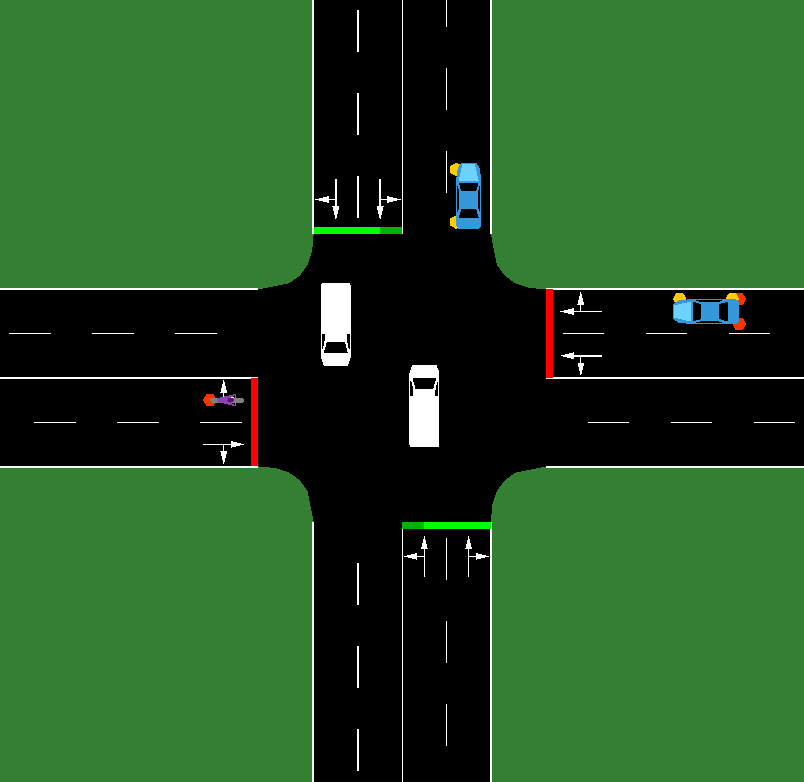
\includegraphics[width=\textwidth]{sumo_manhattan_intersection.png}
        \caption{Dettaglio di un incrocio semaforizzato.}
    \end{subfigure}
    \caption{Scenario Manhattan $8\times8$ visualizzato in SUMO.}
    \label{fig:manhattan-sumo}
\end{figure}

Ogni semaforo possiede due logiche. \texttt{program0}, usato da
\texttt{fixed\_program0}, segue un ciclo statico:
\(42 + 3 + 3 + 42 + 3 + 3 = 96\) secondi. La seconda logica mantiene le stesse
transizioni, ma lascia il cambio fase al controller Max-Pressure. I 30 secondi
di verde principale al posto dei 42 riguardano solo \texttt{fixed\_tuned}.

\section{Configurazione sperimentale}

La campagna finale è identificata da
\texttt{run\_0023\_20260612\_131724}\footnote{I risultati completi della run
sono disponibili nel repository in
\path{logs/ablation/runs/run_0023_20260612_131724}: in particolare
\path{table.txt}, \path{summary_by_group.csv}, \path{summary_vs_base.csv} e
\path{run_results.csv}.}. Comprende una mappa, una distribuzione
uniforme, tre domande, cinque seed e nove scenari:

\begin{equation}
    1\times1\times3\times5\times9=135\text{ simulazioni}.
\end{equation}

Le partenze sono distribuite uniformemente nei primi 3600 secondi. Low contiene
2400 veicoli, medium 4000 e high 5600. Non è imposto un numero massimo di passi:
ciascun caso prosegue fino a esaurimento. Tutti i casi sono terminati con
successo; in ciascuno il numero di viaggi completati coincide con quello
pianificato e la censura è zero. Non sono stati rilevati nei log avvisi di
collisione, teletrasporto o frenata d'emergenza.

La \cref{tab:manhattan-scenarios} riassume gli scenari. I valori non sono tutte
le combinazioni provate durante lo sviluppo, ma una configurazione definitiva
per ogni famiglia.

\begin{table}[htbp]
    \centering
    \caption{Scenari della campagna Manhattan.}
    \label{tab:manhattan-scenarios}
    \begin{tabularx}{\textwidth}{lX}
        \toprule
        Scenario & Configurazione caratterizzante \\
        \midrule
        \texttt{fixed\_program0} & Programma statico \texttt{program0} della mappa \\
        \texttt{mp\_base} & Minimo 10 s, massimo 120 s, margine nullo \\
        \texttt{mp\_lta\_g060\_sf050} & $\gamma=0{,}60$, $s=0{,}50$ veicoli/s \\
        \texttt{mp\_nmin\_a080\_f2} & $\alpha=0{,}80$, floor 2, minimo 4 s, $g=0{,}25$ \\
        \texttt{mp\_downstream\_b04} & $\beta=0{,}4$, EMA $\eta=0{,}30$ \\
        \texttt{mp\_spillback\_on90\_off80} & Soglie 0,90/0,80, almeno 3 veicoli fermi \\
        \texttt{mp\_fair\_mu5\_w20} & $\mu=5$, $w_{1/2}=20$ s \\
        \texttt{mp\_platoon\_x4} & Headway e gap 2,1 s, estensione massima 4 s \\
        \texttt{mp\_switch\_rel005} & Margine relativo 5\% \\
        \bottomrule
    \end{tabularx}
\end{table}

\section{Confronto tra Max-Pressure e controllo fisso}

La campagna Manhattan conferma il risultato più netto della tesi: tutte le
varianti Max-Pressure riducono l'attesa rispetto al programma fisso. Il
\texttt{mp\_base} riduce l'attesa del 59,46\%, 55,93\% e 52,66\% nei tre
livelli; il miglior specialista raggiunge 64,26\%, 60,09\% e 53,05\%. La
\cref{fig:manhattan-reduction} riassume il confronto senza riportare nel testo
tutte le combinazioni numeriche generate dalla pipeline.

\begin{figure}[htbp]
    \centering
    \begin{tikzpicture}
    \begin{axis}[
        ybar,
        width=0.90\textwidth,
        height=7.0cm,
        symbolic x coords={Low,Medium,High},
        xtick=data,
        ymin=0,
        ymax=70,
        ylabel={Riduzione attesa rispetto a \texttt{fixed\_program0} [\%]},
        xlabel={Livello di domanda},
        bar width=12pt,
        enlarge x limits=0.25,
        grid=major,
        legend style={at={(0.5,-0.20)},anchor=north,legend columns=2},
        nodes near coords,
        every node near coord/.append style={font=\scriptsize}
    ]
        \addplot coordinates {(Low,59.46) (Medium,55.93) (High,52.66)};
        \addlegendentry{\texttt{mp\_base}}
        \addplot coordinates {(Low,64.26) (Medium,60.09) (High,53.05)};
        \addlegendentry{Migliore MP}
    \end{axis}
    \end{tikzpicture}
    \caption{Riduzione percentuale del tempo medio di attesa su Manhattan.}
    \label{fig:manhattan-reduction}
\end{figure}

Lo scenario migliore è \texttt{mp\_nmin\_a080\_f2} in low e medium, mentre in
high è \texttt{mp\_fair\_mu5\_w20}. Il valore assoluto dell'attesa passa da
65,85 a 23,54 secondi in low, da 66,89 a 26,70 in medium e da 67,75 a 31,81 in
high. La censura è nulla in tutti i casi, quindi il confronto non dipende da
viaggi incompleti.

Anche i percentili alti confermano il miglioramento: il 95-esimo percentile
scende da 137,22 a 48,00 secondi in low, da 138,80 a 54,20 in medium e da
141,00 a 66,00 in high. Il risparmio medio rispetto al piano statico è ampio:
42,31 secondi in low, 40,20 in medium e 35,94 in high.

\section{Valutazione delle singole estensioni}

Il confronto con \texttt{fixed\_program0} dimostra il valore del controllo
adattivo nella griglia, ma non implica che ogni estensione migliori
\texttt{mp\_base}. In Manhattan molte varianti restano molto vicine tra loro:
questo non le rende inutili, ma indica che la domanda uniforme non evidenzia
tutti i fenomeni per cui sono state progettate.

\subsection{Effetto chiaro: Nmin}

Nmin è l'estensione con il comportamento più distinguibile. Produce il miglior
risultato in low e medium, con un risparmio su \texttt{mp\_base} di 3,16 e 2,78
secondi. In high il vantaggio scende a 0,04 secondi, quindi è trascurabile
rispetto alla variabilità tra seed.

I passi di hold Nmin sono in media 0 in low, 2,4 in medium e 23,2 in high. Il
guadagno a basso traffico non nasce quindi dall'hold dinamico, ma soprattutto
dal minimo verde ridotto a 4 secondi. In high l'hold entra in funzione, ma il
beneficio sull'attesa è minimo e il tempo di viaggio peggiora leggermente.

\subsection{Varianti quasi equivalenti a \texttt{mp\_base}}

Anti-spillback e margine relativo producono gli stessi valori di
\texttt{mp\_base} fino alla precisione dei report. Nel primo caso nessuna corsia
raggiunge contemporaneamente il punteggio 0,90 e almeno tre veicoli fermi; nel
secondo caso il 5\% di banda morta non modifica le decisioni già prese dal
controller.

Anche platoon e fairness restano molto vicini a \texttt{mp\_base}. Platoon rileva
arrivi compatti e aumenta i passi estesi al crescere della domanda, ma il
vantaggio massimo sull'attesa è inferiore a 0,2 secondi. Fairness diventa
nominalmente la migliore in high, ma con soli 0,26 secondi di margine su
\texttt{mp\_base}. Queste differenze sono troppo piccole per parlare di una
superiorità stabile.

\subsection{Varianti penalizzate dalla domanda uniforme}

LTA e penalità downstream peggiorano rispetto a \texttt{mp\_base}. LTA introduce
un margine prudenziale contro gli switch frequenti, ma nella griglia uniforme le
pressioni sono abbastanza regolari e il costo della prudenza supera il beneficio.
La penalità downstream, invece, non trova un vero regime di blocco a valle:
reagisce a occupazioni normali e altera la scelta delle fasi senza prevenire uno
spillback reale.

Questa lettura delimita il significato della campagna Manhattan. Anche 5600
veicoli con domanda uniforme sono sufficienti per confrontare Max-Pressure e
piano fisso, ma non per valutare in modo completo estensioni pensate per code
localizzate, corridoi dominanti, picchi temporali o saturazione a valle. Per
questo la campagna permette di individuare i primi limiti dello scenario
sperimentale Manhattan: il traffico è troppo omogeneo per mettere in crisi alcune
estensioni. Nei capitoli successivi questi problemi vengono affrontati su
Bologna, dove la topologia reale e le distribuzioni skewed e peak rendono il
traffico più concentrato e variabile.

\section{Analisi dei contatori di attivazione}

La \cref{tab:activation-manhattan} riassume i contatori più utili per
interpretare le varianti. Le unità sono passi o eventi medi per simulazione;
per \texttt{mp\_base} viene riportata la coppia switch da margine/interventi da
massimo verde.

\begin{table}[htbp]
    \centering
    \caption{Contatori medi di attivazione per simulazione.}
    \label{tab:activation-manhattan}
    \begin{tabular}{lrrr}
        \toprule
        Meccanismo & Low & Medium & High \\
        \midrule
        \texttt{mp\_base}: switch / max-green & 6071 / 91 & 8591 / 40 & 10184 / 21 \\
        LTA: switch / max-green & 5273 / 260 & 7566 / 158 & 9106 / 90 \\
        Nmin: passi di hold & 0,0 & 2,4 & 23,2 \\
        Fairness: bonus positivi & 5584 & 7951 & 9538 \\
        Spillback: passi bloccati & 0,0 & 0,0 & 0,0 \\
        Platoon: passi estesi & 113,6 & 227,0 & 288,8 \\
        \bottomrule
    \end{tabular}
\end{table}

I contatori evitano due letture superficiali. Una regola può attivarsi spesso
senza migliorare, come fairness e platoon; oppure può non attivarsi affatto,
come spillback e margine relativo. In entrambi i casi il risultato numerico
diventa interpretabile, invece di restare una semplice classifica.

\section{Confronto complessivo}

La campagna supporta con chiarezza l'ipotesi principale: su Manhattan
$8\times8$ con domanda uniforme, il controllo Max-Pressure riduce in modo ampio attesa,
viaggio e time loss rispetto a \texttt{program0} nativo, mantenendo censura nulla. Il
\texttt{mp\_base} da solo riduce l'attesa del 59,46\%, 55,93\% e 52,66\% nei
tre livelli. Non è quindi necessario un modulo specialistico per ottenere il
beneficio fondamentale.

Tra le estensioni, Nmin è la scelta più efficace a domanda bassa e media,
principalmente grazie al minimo verde più corto. A domanda alta fairness,
platoon, Nmin e \texttt{mp\_base} sono compresi entro 0,26 secondi di attesa. La classifica
nominale non deve oscurare tale prossimità. LTA e downstream mostrano invece
che aggiungere prudenza o informazione non produce automaticamente una politica
migliore: una regola utile in congestione può costare capacità quando il
fenomeno bersaglio è assente.

Il piano \texttt{fixed\_program0} rimane quasi costante tra 65,85 e 67,75 secondi di attesa. Ciò
non significa che il traffico non aumenti: viaggio e time loss peggiorano e la
velocità scende. Significa piuttosto che il ciclo statico impone una componente dominante
di ritardo anche in low, mentre il Max-Pressure evita verdi assegnati a
movimenti con poca domanda. La rete regolare e l'assenza di offset coordinati
favoriscono questo vantaggio locale. Non si può estendere la conclusione a un
piano fisso ottimizzato per ogni profilo di domanda.

\section{Indicazioni ricavate per lo scenario reale}

La campagna Manhattan chiarisce il ruolo del Max-Pressure di base: è già un
riferimento forte e ogni estensione deve giustificare il proprio costo. Nmin
mostra che ridurre il minimo verde può essere molto efficace quando il traffico
è leggero, ma anche che il guadagno non coincide sempre con l'hold dinamico
della formula. Spillback, al contrario, non può essere valutato davvero se la
domanda non produce code a valle sufficientemente critiche.

Da questi risultati nasce il passaggio a Bologna. La griglia regolare dimostra
che il controllo adattivo può funzionare, ma non riproduce corridoi dominanti,
picchi temporali e programmi semaforici già calibrati sulla topologia. Nella
rete reale il problema diventa quindi più selettivo: capire quando convenga
usare Max-Pressure, quando conservare il piano nativo e quando attivare una
variante specialistica.

\printbibliography[heading=bibintoc,title={Riferimenti bibliografici}]

\end{document}
